% **************************************************************************************************
% ** SPSC Report and Thesis Template
% **************************************************************************************************
%
% ***** Authors *****
% Daniel Arnitz, Paul Meissner, Stefan Petrik
% Signal Processing and Speech Communication Laboratory (SPSC)
% Graz University of Technology (TU Graz), Austria
%
% ***** Changelog *****
% 0.1   2010-01-25   extracted from report template by Daniel Arnitz (not ready yet)
% 0.2   2010-02-08   added thesis titlepage and modified layout (not ready yet)
% 0.3   2010-02-18   added TUG logo and statutory declaration
% 0.4   2010-02-18   moved the information fields below % **************************************************************************************************
% ** SPSC Report and Thesis Template
% **************************************************************************************************
%
% ***** Authors *****
% Daniel Arnitz, Paul Meissner, Stefan Petrik
% Signal Processing and Speech Communication Laboratory (SPSC)
% Graz University of Technology (TU Graz), Austria
%
% ***** Changelog *****
%
% ***** Todo *****
%
% **************************************************************************************************



\documentclass[%
a4paper,% !!! ATTENTION: geometry package below !!!
\Twosided,% !!! ATTENTION: geometry package below !!!
openany,% begin chapters with new right page (openright) or don't care (openany)
11pt,%
fleqn,% equations not centered, but on the left side
tablecaptionbelow,% captions below tables
% titlepage,% use title
pointlessnumbers,% do not generate point at the end of section numbers (e.g. 1.4.5 instead of 1.4.5.)
final,%
]{scrreprt}% (KOMA)

\usepackage[paper=a4paper,\Twosided,%
textheight=246mm,%
textwidth=160mm,%
heightrounded=true,% round textheight to multiple of lines (avoids overfull vboxes)
ignoreall=true,% do not include header, footer, and margins in calculations
marginparsep=5pt,% marginpar only used for signs (centered), thus only small sep. needed
marginparwidth=10mm,% prevent margin notes to be out of page
hmarginratio=2:1,% set margin ration (inner:outer for twoside) - (2:3 is default)
]{geometry}%


% master
\usepackage{ifthen}% for optional parts
\usepackage[utf8]{inputenc}% German special characters
\ifthenelse{\equal{\DocumentLanguage}{en}}{\usepackage[USenglish]{babel}}{}%
\ifthenelse{\equal{\DocumentLanguage}{de}}{\usepackage[ngerman]{babel}}{}%
\usepackage[%
headtopline,plainheadtopline,% activate all lines (header and footer)
headsepline,plainheadsepline,%
footsepline,plainfootsepline,%
footbotline,plainfootbotline,%
automark% auto update \..mark
]{scrpage2}% (KOMA)
\usepackage{makeidx}% used to make an index directory
\usepackage[]{caption}% customize captions
\usepackage{multicol}%
\usepackage[stable,bottom,hang,splitrule,multiple,symbol*]{footmisc}% customize footnotes


% text
\usepackage{varioref}% improved references
\usepackage{color}% e.g., for color boxes
\usepackage{rotating}% to rotate objects
\usepackage{gensymb}% symbols (perthousand, Celsius, ...)
\usepackage[right]{eurosym}% euro symbol on the right side (51 EUR)
\usepackage[normalem]{ulem}% cross-out, strike-out, underlines (normalem: keep \emph italic)
%\usepackage[safe]{textcomp}% loading in safe mode to avoid problems (see LaTeX companion)
%\usepackage[geometry,misc]{ifsym}% technical symbols
\usepackage{remreset}%\@removefromreset commands (e.g., for continuous footnote numbering)
\usepackage[%
breaklinks=true,% allow line break in links
colorlinks=true,% if false: framed link
linkcolor=black,anchorcolor=black,citecolor=black,filecolor=black,%
menucolor=black,urlcolor=black]{hyperref}% hyperlinks for references


% math
\usepackage{amsmath,amssymb,amstext,bm} % use math packages
\usepackage{mathcomp}% symbols (perthousand, ...) in math mode


% graphics
\usepackage{graphicx}% use simple graphics
\usepackage{subfigure}% subfigures (a),(b),(c)... within figures
\usepackage{flafter}% place floats always after reference
\usepackage{placeins}% preventing floats from crossing a barrier
\usepackage{float}% to place floats !HERE!
\usepackage{psfrag}% replace text in eps figures


% tables
\usepackage{hhline}% hline doesn't work with colored columns, so using hhline
\usepackage{longtable}% for tables longer than one page
\usepackage{dcolumn}% for number alignment in tables
\usepackage{colortbl}% color in tables


% listings
%\usepackage{alltt}% verbatim environment with commands available
\usepackage{listings}% program code listings


% other
%\usepackage{layout}% graphical page layout (spacings)
\usepackage{xspace}% add space after macros if not followed by punctuation character
\makeindex% used for index creation

 (encoding...)
% 0.5   2010-03-02   added \ShortTitle to fix problems with long thesis titles
%                    added \ThesisType (makes the template suitable for MSc, BSc, PhD, ... Thesis)
%
% ***** Todo *****
% - Introduction/Usage
% **************************************************************************************************

% **************************************************************************************************
% basic setup
\newcommand{\DocumentType}{report} % "thesis" / "report"
\newcommand{\DocumentLanguage}{de} % "en" / "de"
\newcommand{\Twosided}{} % "twoside" / ""


% **************************************************************************************************
% template setup -- do not change these unless you know what you are doing!
% **************************************************************************************************
% ** SPSC Report and Thesis Template
% **************************************************************************************************
%
% ***** Authors *****
% Daniel Arnitz, Paul Meissner, Stefan Petrik
% Signal Processing and Speech Communication Laboratory (SPSC)
% Graz University of Technology (TU Graz), Austria
%
% ***** Changelog *****
%
% ***** Todo *****
%
% **************************************************************************************************



\documentclass[%
a4paper,% !!! ATTENTION: geometry package below !!!
\Twosided,% !!! ATTENTION: geometry package below !!!
openany,% begin chapters with new right page (openright) or don't care (openany)
11pt,%
fleqn,% equations not centered, but on the left side
tablecaptionbelow,% captions below tables
% titlepage,% use title
pointlessnumbers,% do not generate point at the end of section numbers (e.g. 1.4.5 instead of 1.4.5.)
final,%
]{scrreprt}% (KOMA)

\usepackage[paper=a4paper,\Twosided,%
textheight=246mm,%
textwidth=160mm,%
heightrounded=true,% round textheight to multiple of lines (avoids overfull vboxes)
ignoreall=true,% do not include header, footer, and margins in calculations
marginparsep=5pt,% marginpar only used for signs (centered), thus only small sep. needed
marginparwidth=10mm,% prevent margin notes to be out of page
hmarginratio=2:1,% set margin ration (inner:outer for twoside) - (2:3 is default)
]{geometry}%


% master
\usepackage{ifthen}% for optional parts
\usepackage[utf8]{inputenc}% German special characters
\ifthenelse{\equal{\DocumentLanguage}{en}}{\usepackage[USenglish]{babel}}{}%
\ifthenelse{\equal{\DocumentLanguage}{de}}{\usepackage[ngerman]{babel}}{}%
\usepackage[%
headtopline,plainheadtopline,% activate all lines (header and footer)
headsepline,plainheadsepline,%
footsepline,plainfootsepline,%
footbotline,plainfootbotline,%
automark% auto update \..mark
]{scrpage2}% (KOMA)
\usepackage{makeidx}% used to make an index directory
\usepackage[]{caption}% customize captions
\usepackage{multicol}%
\usepackage[stable,bottom,hang,splitrule,multiple,symbol*]{footmisc}% customize footnotes


% text
\usepackage{varioref}% improved references
\usepackage{color}% e.g., for color boxes
\usepackage{rotating}% to rotate objects
\usepackage{gensymb}% symbols (perthousand, Celsius, ...)
\usepackage[right]{eurosym}% euro symbol on the right side (51 EUR)
\usepackage[normalem]{ulem}% cross-out, strike-out, underlines (normalem: keep \emph italic)
%\usepackage[safe]{textcomp}% loading in safe mode to avoid problems (see LaTeX companion)
%\usepackage[geometry,misc]{ifsym}% technical symbols
\usepackage{remreset}%\@removefromreset commands (e.g., for continuous footnote numbering)
\usepackage[%
breaklinks=true,% allow line break in links
colorlinks=true,% if false: framed link
linkcolor=black,anchorcolor=black,citecolor=black,filecolor=black,%
menucolor=black,urlcolor=black]{hyperref}% hyperlinks for references


% math
\usepackage{amsmath,amssymb,amstext,bm} % use math packages
\usepackage{mathcomp}% symbols (perthousand, ...) in math mode


% graphics
\usepackage{graphicx}% use simple graphics
\usepackage{subfigure}% subfigures (a),(b),(c)... within figures
\usepackage{flafter}% place floats always after reference
\usepackage{placeins}% preventing floats from crossing a barrier
\usepackage{float}% to place floats !HERE!
\usepackage{psfrag}% replace text in eps figures


% tables
\usepackage{hhline}% hline doesn't work with colored columns, so using hhline
\usepackage{longtable}% for tables longer than one page
\usepackage{dcolumn}% for number alignment in tables
\usepackage{colortbl}% color in tables


% listings
%\usepackage{alltt}% verbatim environment with commands available
\usepackage{listings}% program code listings


% other
%\usepackage{layout}% graphical page layout (spacings)
\usepackage{xspace}% add space after macros if not followed by punctuation character
\makeindex% used for index creation


\input{./base/layout_\DocumentType}
% **************************************************************************************************
% ** SPSC Report and Thesis Template
% **************************************************************************************************
%
% ***** Authors *****
% Daniel Arnitz, Paul Meissner, Stefan Petrik
% Signal Processing and Speech Communication Laboratory (SPSC)
% Graz University of Technology (TU Graz), Austria
%
% ***** Changelog *****
%
% ***** Todo *****
%
% **************************************************************************************************



% **************************************************************************************************
% * SECTIONING AND TEXT
% **************************************************************************************************

% new chapter, section, ... plus a few addons
%   part
\newcommand{\newpart}[2]{\FloatBarrier\cleardoublepage\part{#1}\label{part:#2}}%
%   chapter
\newcommand{\newchapter}[2]{\FloatBarrier\chapter{#1}\label{chp:#2}}
\newcommand{\newchapterNoTOC}[2]{\FloatBarrier\stepcounter{chapter}\chapter*{#1}\label{chp:#2}}%
%   section
\newcommand{\newsection}[2]{\FloatBarrier\vspace{5mm}\section{#1}\label{sec:#2}}%
\newcommand{\newsectionNoTOC}[2]{\FloatBarrier\vspace{5mm}\stepcounter{section}\section*{#1}\label{sec:#2}}%
%   subsection
\newcommand{\newsubsection}[2]{\FloatBarrier\vspace{3mm}\subsection{#1}\label{sec:#2}}%
\newcommand{\newsubsectionNoTOC}[2]{\FloatBarrier\vspace{3mm}\stepcounter{subsection}\subsection*{#1}\label{sec:#2}}%
%   subsubsection
\newcommand{\newsubsubsection}[2]{\vspace{2mm}\subsubsection{#1}\label{sec:#2}}%
\newcommand{\newsubsubsectionNoTOC}[2]{\vspace{2mm}\stepcounter{subsubsection}\subsubsection*{#1}\label{sec:#2}}%

% next paragraph
\newcommand{\nxtpar}{\par\bigskip}

% "stylish" quotes on the right side
\newcommand{\openingquote}[2]{\hfill\parbox[t]{10cm}{\itshape\raggedleft{"#1"}\\\footnotesize -- #2}\nxtpar}%

% direct quotes
% \newenvironment{directquote}{\nxtpar\hrule}{\hrule}\hfill\litref{#1}{#2}}

% warnings and attention signs in marginpar
\newcommand{\MDanger}{\marginpar{\Huge\centering\fbox{\textbf{!}}}}%
\newcommand{\MAttention}{\marginpar{\Huge\centering\textbf{!}}}%
\newcommand{\MHint}{\marginpar{\Huge\centering\textbf{\checkmark}}}%
\newcommand{\MQuestion}{\marginpar{\Huge\centering\textbf{?}}}%

% same footnote number as last one
\newcommand{\lastfootnotemark}{\addtocounter{footnote}{-1}\footnotemark}%

% value-unit commands (for 457 kHz, etc)
\newcommand{\vu}[2]{\mbox{$#1\,\text{#2}$}} % "value~unit" ... prevents e.g. 456 \linebreak mV
\newcommand{\vuc}[3]{\mbox{$#1\,\text{#2}\;#3\,\%$}} % "value~unit~tolerance-per-cent"
\newcommand{\vum}[3]{\mbox{$#1\,\text{#2}\;#3\,\perthousand$}} % "value~unit~tolerance-per-mil"

% reminders
\newcommand{\reminder}[1]{\colorbox{red}{#1}\xspace}%
\newcommand{\rem}{\reminder{(...)}}%
\newcommand{\remq}{\reminder{???}}%
\newcommand{\uc}{\nxtpar\colorbox{yellow}{... under construction ...}\nxtpar}%

% misc
\newcommand{\pwd}{.} % present working directory (can be used to create relativ paths per part, etc.)


% **************************************************************************************************
% * MATH
% **************************************************************************************************

% highlighting
\newcommand{\vm}[1]{\bm{#1}}% vector or matrix

% operators
\newcommand{\E}[1]{\text{E}\!\left\{#1\right\}}% expectation operator
\newcommand{\var}[1]{\text{var}\!\left\{#1\right\}}% variance operator
\renewcommand{\ln}[1]{\text{ln}\!\left(#1\right)}% natural logarithm
\newcommand{\ld}[1]{\text{ld}\!\left(#1\right)}% logarithm base 2
\renewcommand{\log}[1]{\text{log}\!\left(#1\right)}% logarithm (base 10)
\newcommand{\logb}[2]{\text{log}_{#1}\!\left(#2\right)}% logarithm base ...
\newcommand{\avgvar}[1]{\overline{\text{var}}\!\left\{#1\right\}}% average variance operator
\renewcommand{\Re}[1]{\text{Re}\!\left\{#1\right\}}% real part
\renewcommand{\Im}[1]{\text{Im}\!\left\{#1\right\}}% imaginary part

% other
\newcommand{\conj}{^\ast}% conjugate complex
\newcommand{\mtx}[2]{\left[\begin{array}{#1}#2\end{array}\right]}%vector/matrix


% **************************************************************************************************
% * FLOATS (FIGURES, TABLES, LISTINGS, ...)
% **************************************************************************************************

% figures without frames
%   standard
\newcommand{\fig}[3]{\begin{figure}\centering\includegraphics[width=\textwidth]{#1}\caption{#2}\label{fig:#3}\end{figure}}%
%   with controllable parameters
\newcommand{\figc}[4]{\begin{figure}\centering\includegraphics[#1]{#2}\caption{#3}\label{fig:#4}\end{figure}}%
%   two subfigures
\newcommand{\twofig}[6]{\begin{figure}\centering%
\subfigure[#2]{\includegraphics[width=0.495\textwidth]{#1}}%
\subfigure[#4]{\includegraphics[width=0.495\textwidth]{#3}}%
\caption{#5}\label{fig:#6}\end{figure}}%
%   two subfigures and controllable parameters
\newcommand{\twofigc}[8]{\begin{figure}\centering%
\subfigure[#3]{\includegraphics[#1]{#2}}%
\subfigure[#6]{\includegraphics[#4]{#5}}%
\caption{#7}\label{fig:#8}\end{figure}}%

% framed figures
%   standard
\newcommand{\figf}[3]{\begin{figure}\centering\fbox{\includegraphics[width=\textwidth]{#1}}\caption{#2}\label{fig:#3}\end{figure}}%
%   with controllable parameters
\newcommand{\figcf}[4]{\begin{figure}\centering\fbox{\includegraphics[#1]{#2}}\caption{#3}\label{fig:#4}\end{figure}}%
%   two subfigures
\newcommand{\twofigf}[6]{\begin{figure}\centering%
\fbox{\subfigure[#2]{\includegraphics[width=0.495\textwidth]{#1}}}%
\fbox{\subfigure[#4]{\includegraphics[width=0.495\textwidth]{#3}}}%
\caption{#5}\label{fig:#6}\end{figure}}%
%   two subfigures and controllable parameters
\newcommand{\twofigcf}[8]{\begin{figure}\centering%
\fbox{\subfigure[#3]{\includegraphics[#1]{#2}}}%
\fbox{\subfigure[#6]{\includegraphics[#4]{#5}}}%
\caption{#7}\label{fig:#8}\end{figure}}%

% listings
\newcommand{\filelisting}[4]{\lstinputlisting[print=true,language=#1,caption={#3},label={lst:#4}]{#2}}

% preserve backslash for linebreaks in tables (ragged... redefines \\, thus it has to be preserved)
\newcommand{\pbs}[1]{\let\temp=\\#1\let\\=\temp}%

\graphicspath{{./drawings/}{./plots/}{./images/}}
% **************************************************************************************************
% ATTENTION: Make sure that makeindex is set to -s "./base/index.sty"
% **************************************************************************************************

% uncomment to get watermarks:
% \usepackage[first,bottom,light,draft]{draftcopy}
% \draftcopyName{ENTWURF}{160}


% **************************************************************************************************
% information fields

% general
\newcommand{\DocumentTitle}{Computational Intelligence UE}
\newcommand{\DocumentSubtitle}{Homework 2: Backpropagation and Neural Networks}
\newcommand{\ShortTitle}{CI Homework 2} % used in headers (keep short!)
\newcommand{\DocumentAuthor}{Thomas Ebner, Raphael Hoheneder, Stefan N\"ohmer}
\newcommand{\DocumentDate}{Graz, \today}
%    for thesis only (will be ignored for reports)
\newcommand{\ThesisType}{Master's Thesis}
\newcommand{\Organizations}{Signal Processing and Speech Communications Laboratory \\ Graz University of Technology \\[1cm] on behalf of \\ Some Company} % SPSC \\ TUG \\[1cm] on behalf of \\ A Nice Company
\newcommand{\Advisors}{Dipl.-Ing. Dr. Assoc.Prof. Klaus Witrisal \\ Dipl.-Ing. Paul Meissner} % Advisor 1 \\ Advisor 2 \\ ...
\newcommand{\Supervisors}{Univ.-Prof. Dipl.-Ing. Dr.techn. Gernot Kubin}

% revision number
\newcommand{\RevPrefix}{alpha~}
\newcommand{\RevLarge}{1}
\newcommand{\RevSmall}{1}

% confidential?
\newcommand{\ConfidNote}{confidential}% {"confidential", "eyes only", ...}

% short command for vectors
\newcommand{\vect}[1]{\mathbf{#1}}


\begin{document}

%listingstyle:
\definecolor{orange}{rgb}{0.75,0.65,0}
\definecolor{gruen}{rgb}{0,0.5,0}
\definecolor{listinggray}{gray}{0.97}
\definecolor{listingshadow}{gray}{0.2}
\lstloadlanguages{Matlab}
\lstset{frame=shadowbox,
		rulesepcolor=\color{listingshadow},
		numbers=left,
		basicstyle=\scriptsize\ttfamily,
		numberstyle=\tiny,
		keywordstyle=\color{blue}\bfseries, % bold black keywords
		identifierstyle=, % nothing happens
		commentstyle=\color{gruen}, % comments
		stringstyle=\color{orange}, % typewriter type for strings
		showstringspaces=false,
		tabsize=4,
		backgroundcolor=\color{listinggray}
        }

% **************************************************************************************************
% titlepage
\input{./base/titlepage_\DocumentType}

% statutory declaration for theses
\ifthenelse{\equal{\DocumentType}{thesis}}{% **************************************************************************************************
% ** SPSC Report and Thesis Template
% **************************************************************************************************
%
% ***** Authors *****
% Daniel Arnitz, Paul Meissner, Andreas Laesser, Stefan Petrik
% Signal Processing and Speech Communication Laboratory (SPSC)
% Graz University of Technology (TU Graz), Austria
%
% ***** Changelog *****
% 0.1   2010-02-18   created
% 0.2   2010-03-02   added German declaration
%
% ***** Todo *****
% **************************************************************************************************

\cleardoublepage
\pagestyle{empty}\pagenumbering{roman}

\vspace*{1cm}

% English
\ifthenelse{\equal{\DocumentLanguage}{en}}{
\begin{center}\Large\bfseries Statutory Declaration\end{center}\vspace*{1cm}
\noindent I declare that I have authored this thesis independently, that I have not used other than the declared sources$/$resources, and that I have explicitly marked all material which has been quoted either literally or by content from the used sources.
\par\vspace*{4cm}
\centerline{
\begin{tabular}{m{1.5cm}cm{1.5cm}m{3cm}m{1.5cm}cm{1.5cm}}
\cline{1-3} \cline{5-7}
 & date & & & & (signature) &\\
\end{tabular}}
}

% German
\ifthenelse{\equal{\DocumentLanguage}{de}}{
\begin{center}\Large\bfseries Eidesstattliche Erkl�rung\end{center}\vspace*{1cm}
Ich erkl�re an Eides statt, dass ich die vorliegende Arbeit selbstst�ndig verfasst, andere als die angegebenen Quellen$/$Hilfsmittel nicht benutzt, und die den benutzten Quellen w�rtlich und inhaltlich entnommene Stellen als solche kenntlich gemacht habe.
\par\vspace*{4cm}
\centerline{
\begin{tabular}{m{1.5cm}cm{1.5cm}m{3cm}m{1.5cm}cm{1.5cm}}
\cline{1-3} \cline{5-7}
 & Graz, am & & & & (Unterschrift) &\\
\end{tabular}}
}

}{}


% **************************************************************************************************
% **************************************************************************************************
% user-defined part

\chapter{Homework: Backpropagation and Neural Networks}
\section{Backpropagation}
\subsection{Backpropagation for a simple network}

\begin{figure}[hp!]
\begin{center}
 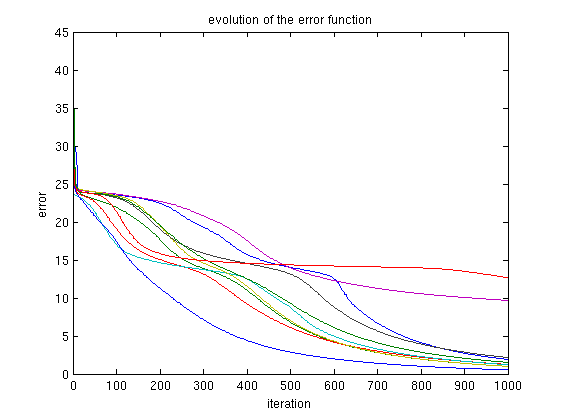
\includegraphics[width=0.99\textwidth]{./figures/1/error}
 \caption{Evolution of the error over the iterations with different startweight-vectors}
\label{fig:backprop_error}
\end{center}
\end{figure}



\begin{figure}[hp!]
\begin{center}
 \begin{minipage}{0.48\textwidth}
 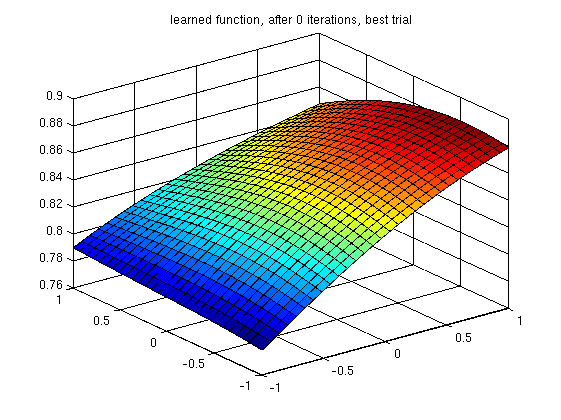
\includegraphics[width=0.99\textwidth]{./figures/1/learned_best_0}
 \end{minipage}
 \begin{minipage}{0.48\textwidth}
 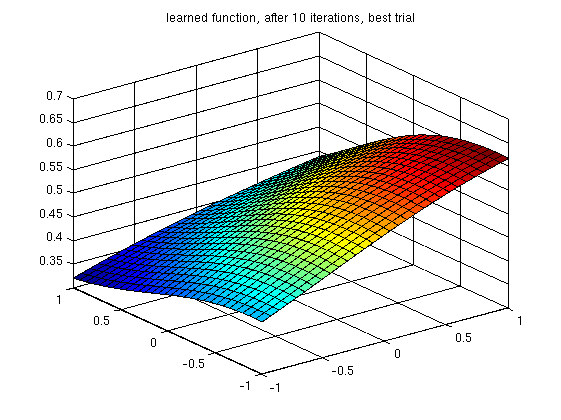
\includegraphics[width=0.99\textwidth]{./figures/1/learned_best_10}
 \end{minipage}
 \begin{minipage}{0.48\textwidth}
 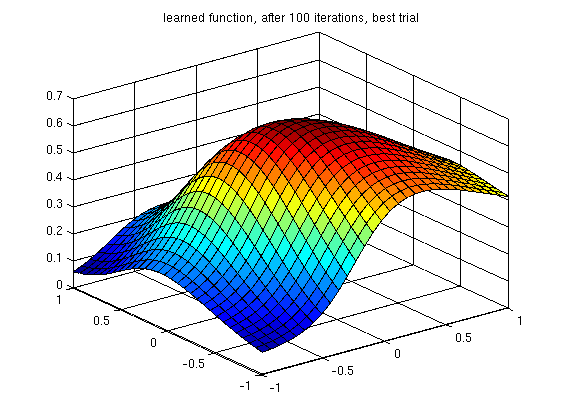
\includegraphics[width=0.99\textwidth]{./figures/1/learned_best_100}
 \end{minipage}
 \begin{minipage}{0.48\textwidth}
 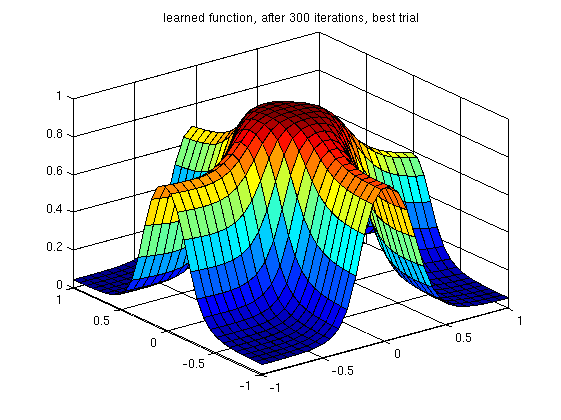
\includegraphics[width=0.99\textwidth]{./figures/1/learned_best_300}
 \end{minipage}
 \begin{minipage}{0.48\textwidth}
 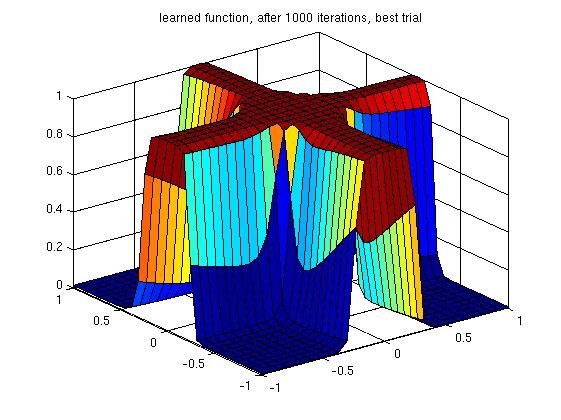
\includegraphics[width=0.99\textwidth]{./figures/1/learned_best_1000}
 \end{minipage}
 \caption{Learned Function after 0,10,100,300,1000 Iterations(Best Trial)}
\label{fig:learned_function_best}
\end{center}
\end{figure}


\begin{figure}[hp!]
\begin{center}
 \begin{minipage}{0.48\textwidth}
 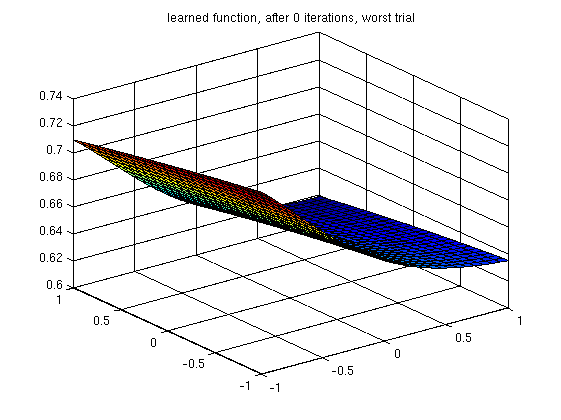
\includegraphics[width=0.99\textwidth]{./figures/1/learned_worst_0}
 \end{minipage}
 \begin{minipage}{0.48\textwidth}
 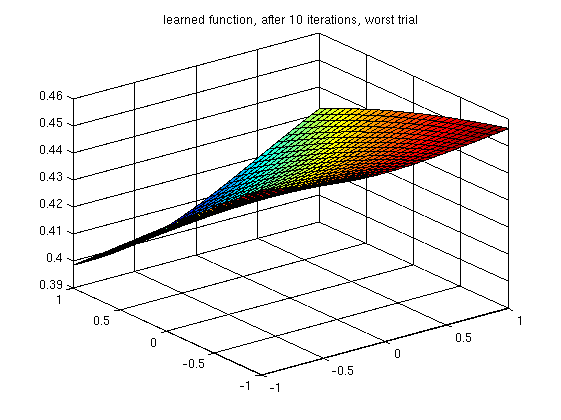
\includegraphics[width=0.99\textwidth]{./figures/1/learned_worst_10}
 \end{minipage}
 \begin{minipage}{0.48\textwidth}
 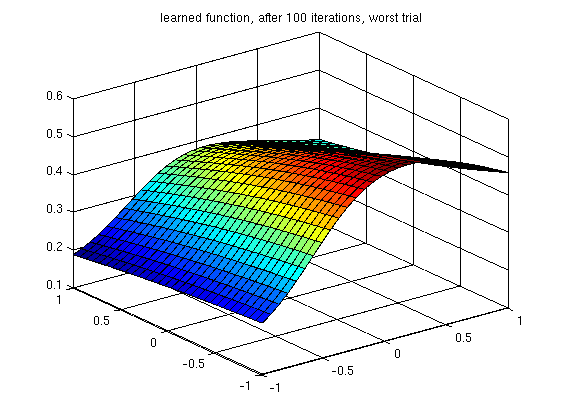
\includegraphics[width=0.99\textwidth]{./figures/1/learned_worst_100}
 \end{minipage}
 \begin{minipage}{0.48\textwidth}
 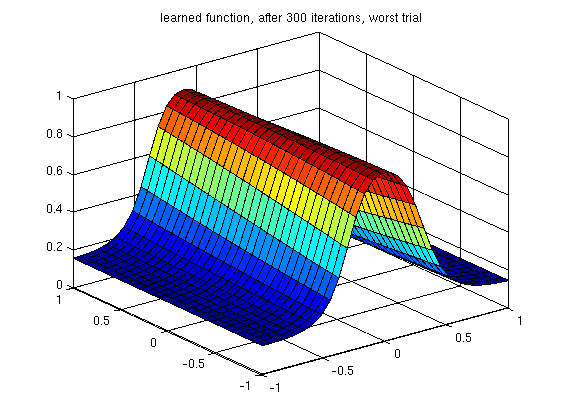
\includegraphics[width=0.99\textwidth]{./figures/1/learned_worst_300}
 \end{minipage}
 \begin{minipage}{0.48\textwidth}
 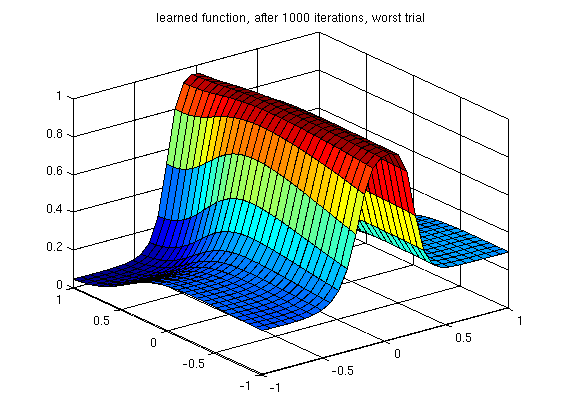
\includegraphics[width=0.99\textwidth]{./figures/1/learned_worst_1000}
 \end{minipage}
 \caption{Learned Function after 0,10,100,300,1000 Iterations(Worst Trial)}
\label{fig:learned_function_worst}
\end{center}
\end{figure}


\clearpage
\newpage
\section{Simple Regression with Neural Networks}
\begin{figure}[h!]
  \centering
  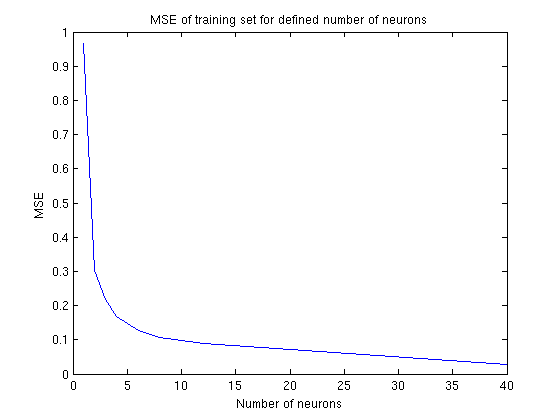
\includegraphics[width=0.75\textwidth]{./figures/3/3_mse_train.png}
  \caption{MSE für unterschiedliche Anzahl an Neuronen des Trainingssets}
  \label{fig:3_mse_train}
\end{figure}

\begin{figure}[h!]
  \centering
  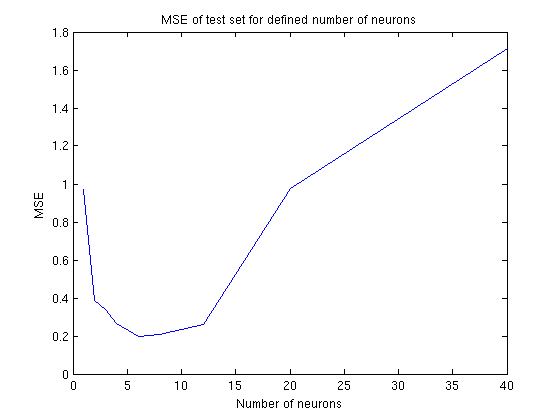
\includegraphics[width=0.75\textwidth]{./figures/3/3_mse_test.png}
  \caption{MSE für unterschiedliche Anzahl an Neuronen des Testsets}
  \label{fig:3_mse_test}
\end{figure}

Abbildungen \ref{fig:3_mse_train} und \ref{fig:3_mse_test} zeigen den Mean Squared Error (MSE) für unterschiedliche Neuronenanzahl bei den Trainings- bzw. Testdatensätzen. Man erkennt, dass der MSE bei den Trainingsdaten immer kleiner wird, je mehr Neuronen verwendet werden, da sich die entstehende Funktion des Neuronalen Netzwerks immer mehr den Trainingsdaten annähert. Betrachtet man allerdings den MSE der Testdaten, erkennt man, dass ab einer bestimmten Neuronenanzahl der Fehler wieder steigt. Dieser Effekt wird als \emph{Overfitting} bezeichnet, da das Neuronale Netzwerk versucht, die Trainingsdaten perfekt nachzubilden. Dadurch stimmt die gelernte Funktion nicht mehr mit der Zielfunktion überein.

Der beste Wert für $n$ wäre in diesem Fall 6, da hier der Fehler bei den Testdaten am geringsten ist. Für größere $n$ tritt Overfitting auf.

\begin{figure}[h!]
  \centering
  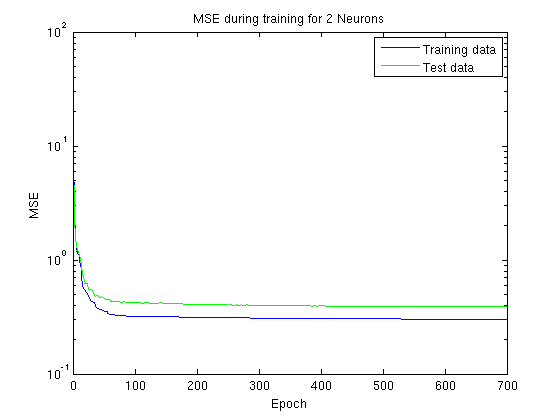
\includegraphics[width=0.7\textwidth]{./figures/3/3_mse_2.png}
  \caption{MSE des Trainings- und Testsets für 2 Neuronen}
  \label{fig:3_mse_2}
\end{figure}

\begin{figure}[h!]
  \centering
  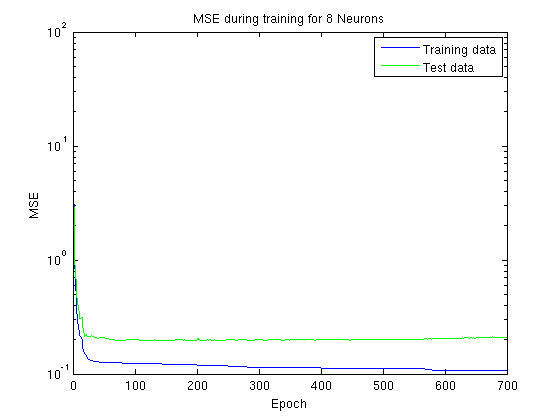
\includegraphics[width=0.7\textwidth]{./figures/3/3_mse_8.png}
  \caption{MSE des Trainings- und Testsets für 8 Neuronen}
  \label{fig:3_mse_8}
\end{figure}

\begin{figure}[h!]
  \centering
  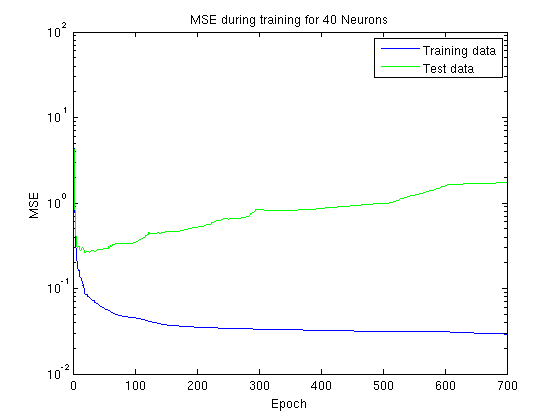
\includegraphics[width=0.7\textwidth]{./figures/3/3_mse_40.png}
  \caption{MSE des Trainings- und Testsets für 40 Neuronen}
  \label{fig:3_mse_40}
\end{figure}

Abbildungen \ref{fig:3_mse_2}, \ref{fig:3_mse_8} und \ref{fig:3_mse_40} zeigen den MSE auf den Trainings- und Testdaten für 2, 8, bzw. 40 Neuronen. Man erkennt, dass es bei niedriger Anzahl an Neuronen (hier: 2, Abb.~\ref{fig:3_mse_2}) keinen Overfitting-Effekt gibt, der verbleibende Fehler auf den Trainings- und Testdaten jedoch relativ hoch bleibt. Bei einer mittleren Anzahl an Neuronen (hier: 8, Abb.~\ref{fig:3_mse_8}) wird der Fehler auf den Trainings- und Testdaten kleiner, jedoch macht sich Overfitting bereits minimal bemerkbar. Bei einer hohen Anzahl an Neuronen (hier: 40, Abb.~\ref{fig:3_mse_40}) wird der Fehler auf den Trainingsdaten zwar sehr klein, durch Overfitting steigt der Fehler auf den Testdaten jedoch wieder stark an.

Der Fehler auf den Trainingsdaten nimmt mit zunehmender Anzahl Neuronen immer weiter ab, da die Funktion der Trainingsdaten immer genauer nachgebildet wird. Der Fehler auf den Testdaten steigt jedoch ab einer gewissen Anzahl Neuronen wieder, da der \emph{Overfitting}-Effekt auftritt.

\begin{figure}[h!]
  \centering
  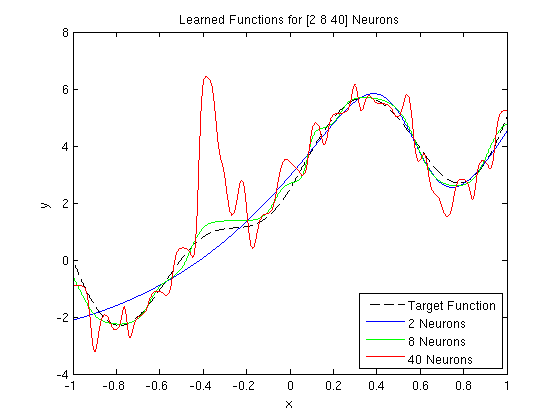
\includegraphics[width=0.75\textwidth]{./figures/3/3_learned.png}
  \caption{gelernte Funktion bei 2, 8 bzw. 40 Neuronen}
  \label{fig:3_learned}
\end{figure}

Abbildung~\ref{fig:3_learned} zeigt die gelernten Funktionen für 2, 8 bzw. 40 Neuronen. Wie man in den vorherigen Plots erkennt, ist die Annäherung an die Zielfunktion mit 2 Neuronen noch relativ schlecht, da der MSE noch sehr groß ist. Bei 8 Neuronen ist der MSE um einiges gesunken, deswegen wird auch die Zielfunktion gut angenähert. Bei zu vielen Neuronen, wie hier 40, tritt der Overfitting-Effekt auf und das Neuronale Netzwerk versucht eine Funktion zu finden, das die Trainingsdaten möglichst gut abbildet. Dadurch entfernt sich die gelernte Funktion wieder von der Zielfunktion.

Hier treten die gleichen Effekte auf wie bei der Linearen Regression. Der Grad des Polynoms hat den gleichen Effekt auf die Qualität der gelernten Funktion wie die Anzahl der Neuronen beim Neuronalen Netzwerk. Ist der Grad zu niedrig, kann die Funktion nicht gut nachgebildet werden. Ist der Grad zu hoch, tritt Overfitting auf.

\clearpage
\subsection{Regularized Neural Networks}

\subsubsection{Weight Decay}

\begin{figure}[h!]
  \centering
  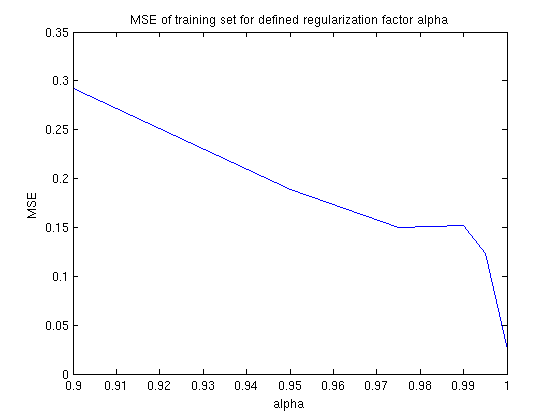
\includegraphics[width=0.75\textwidth]{./figures/3/3_1_mse_train_wd.png}
  \caption{MSE des Trainingssets mit \emph{weight decay} für unterschiedliche $\alpha$}
  \label{fig:3_1_mse_train_wd}
\end{figure}

\begin{figure}[h!]
  \centering
  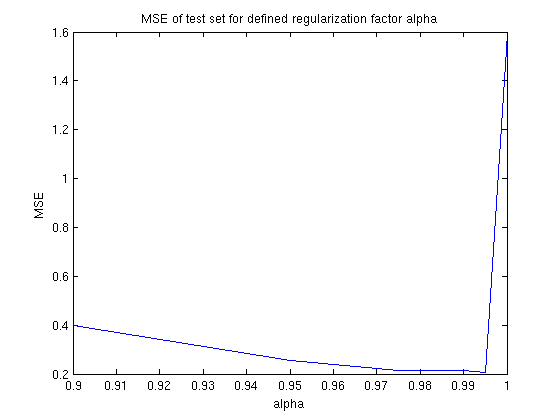
\includegraphics[width=0.75\textwidth]{./figures/3/3_1_mse_test_wd.png}
  \caption{MSE des Testsets mit \emph{weight decay} für unterschiedliche $\alpha$}
  \label{fig:3_1_mse_test_wd}
\end{figure}

Abbildungen \ref{fig:3_1_mse_train_wd} und \ref{fig:3_1_mse_test_wd} zeigen den Fehler des Trainings- bzw. Testsets für unterschiedliche $\alpha$. Bei \emph{weight decay} wird dem MSE ein \emph{penalty term} dazuaddiert, der sich aus den Gewichten berechnet. Dadurch wird bei steigenden Gewichten auch der Fehler größer, was dazu führt, dass Gewichte keine sehr großen Werte annehmen. Dadurch wird verhindert, dass sich die Gewichte zu sehr an die Trainingsdaten anpassen, dadurch wird Overfitting vermindert. Bei kleinem $\alpha$ steigt der Fehler, da die Gewichtssumme zu stark ins Gewicht fällt. Erhöht man $\alpha$, kommt man irgendwann zu dem Wert, bei dem der Fehler minimiert wird, indem die Größe der Gewichte sinnvoll beschränkt wird. Erhöht man dann $\alpha$ weiter, kommt man wieder zum gleichen Ergebnis wie ohne weight decay, nämlich Overfitting.

Bei diesem Beispiel ergab sich der beste Wert zu $\alpha = 0.995$.

\emph{Weight decay} erzielt den gleichen Effekt wie der \emph{regularization term} bei linearer Regression. Bei Betrachtung der Formeln sieht man, dass diese prinzipiell übereinstimmen, nämlich der MSE und die Summe der Gewichte, jeweils wiederum gewichtet.

\begin{figure}[h!]
  \centering
  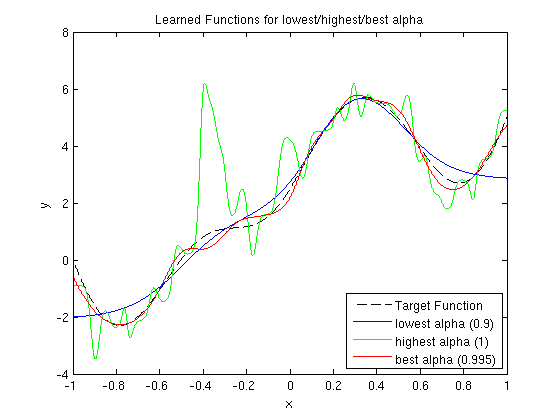
\includegraphics[width=0.75\textwidth]{./figures/3/3_1_learned_wd.png}
  \caption{Gelernte Funktionen mit \emph{weight decay} für das geringste, größte und beste $\alpha$}
  \label{fig:3_1_learned_wd}
\end{figure}

Abbildung~\ref{fig:3_1_learned_wd} zeigt die gelernte Funktion für das geringste, größte und beste $\alpha$. Man erkennt, dass bei zu niedrigem $\alpha$ die Kurve zu ``flach'' ist, da die Gewichte zu stark in den Fehler einfließen. Bei zu hohem $\alpha$ erhält man das gleiche Ergebnis wie ohne weight decay.


\subsubsection{Early Stopping}

\begin{figure}[h!]
  \centering
  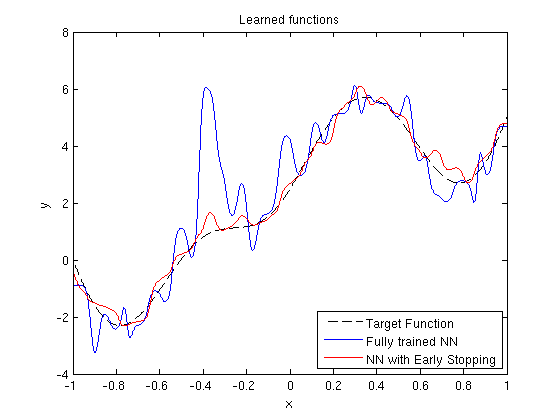
\includegraphics[width=0.75\textwidth]{./figures/3/3_1_learned_es.png}
  \caption{Gelernte Funktionen mit \emph{early stopping} des komplett trainierten Netzwerkes und des Early-Stopped Netzwerkes}
  \label{fig:3_1_learned_es}
\end{figure}

Abbildung \ref{fig:3_1_learned_es} zeigt die gelernte Funktion des komplett trainierten Netzwerkes bzw. des Early-Stopped Netzwerkes. Die gelernte Funktion des komplett trainierten Netzwerkes ist bereits ein vertrautes Bild, sie entspricht der der vorangegangenen Methoden. Beim \emph{early stopping} bricht man den Lernvorgang des Neuronalen Netzwerkes dann ab, wenn der Fehler auf den Testdaten am geringsten ist (also wenn die Gewichte noch ``generell'' genug sind, und es noch nicht zu Overfitting gekommen ist). Dadurch ergibt sich ein sehr geringer Fehler.

Das \textsc{Matlab}-Skript (siehe Anhang) ermittelt den geringsten Fehler auf den Testdaten, und bei welcher Epoche dieser auftritt:

\noindent \texttt{fully trained NN with 40 neurons: 0.028497 mse on training set, 1.572938 mse on testset\\
minimal mse is 0.232383 at epoch 11\\
early stopping trained NN with 40 neurons: 0.137280 mse on training set, 0.232383 mse on testset}


\subsubsection{Comparison}

\paragraph{Different Number of Neurons}

Bei unterschiedlichen Anzahlen von Neuronen treten die genannten Effekte auf: sind die Neuronen zu wenig, kann die geforderte Funktion nur schlecht angenähert werden. Ist die Anzahl der Neuronen zu hoch, kommt es zu Overfitting. Im Beispiel gibt es ein Optimum hinsichtlich der Anzahl der Neuronen, welches bei 6 Neuronen liegt (siehe Abb. \ref{fig:3_mse_test}). Bei den angegebenen Neuronenanzahlen erreicht das NN mit 8 Neuronen den minimalen MSE von ca. 0.21.

\paragraph{Weight Decay}

Für den richtigen Regularisierungsfaktor $\alpha$ wurden bessere Ergebnisse erzielt als mit der vorherigen Methode. Es muss jedoch für jeden möglichen Faktor $\alpha$ das gesamte NN trainiert werden, was sehr zeitaufwändig ist. Durch den Regularisierungsfaktor verhindert man den Overfitting-Effekt. Mit Weight Decay erreicht man einen minimalen MSE von ca. 0.2.

\paragraph{Early Stopping}

Early Stopping erzielt etwas schlechtere Ergebnisse als Weight Decay, dafür muss nur ein NN komplett trainiert werden, und ein weiteres NN nur bis zur optimalen Epoche. Dadurch verringert sich die Rechenzeit drastisch. Mit Early Stopping erreicht man einen minimalen MSE von ca. 0.23.



\clearpage
\newpage

\chapter{Listings}
\section{Backpropagation of neuronal networks}
\lstinputlisting[language=matlab]{../implementation/templateScript.m}
\section{feedforwardNN}
\lstinputlisting[language=matlab]{../implementation/feedforwardNN.m}
\section{backpropNNSingle}
\lstinputlisting[language=matlab]{../implementation/backpropNNSingle.m}
\section{backpropNNFull}
\lstinputlisting[language=matlab]{../implementation/backpropNNFull.m}
\section{Simple Regression with Neural Networks}
\lstinputlisting[language=matlab]{../implementation/ue2_3.m}
\section{Simple Regression with Neural Networks and weight decay}
\lstinputlisting[language=matlab]{../implementation/ue2_3_1_wd.m}
\section{Simple Regression with Neural Networks and early stopping}
\lstinputlisting[language=matlab]{../implementation/ue2_3_1_es.m}





% **************************************************************************************************
% **************************************************************************************************

%\appendix
%\bibliographystyle{/.base/ieeetran}
%\bibliography{_bibliography}

% place all floats and create label on last page
\FloatBarrier\label{end-of-document}
\end{document}

